\documentclass{article}
\usepackage[utf8]{inputenc}

\usepackage[a4paper]{geometry}

\usepackage{amsmath}
\usepackage{amsthm} % theorems, definitions etc.

\usepackage{hyperref} % hyperlinks and pdf contents

\usepackage{graphicx}
\DeclareGraphicsExtensions{.png,.pdf}

\title{Bachelor}
\author{Andreas Matre}
\date{February 2020}

\begin{document}

\newtheorem{definition}{Definition}[subsection]
\newtheorem{theorem}{Theorem}
\newtheorem{example}{Example}[section]


\maketitle

\section{Abstract}

\tableofcontents

\section{Introduction}

Linear regression is a useful tool to describe relationships between variables.
It can for example be used in the social sciences to try to show a relationship
between income and age of death. 

When you want to model a relationship between a response and predictors, you
first need to collect data to fit that model. This data can be collected in many
different ways and it is very important to take into account the methods used in
the information gathering when fitting models. This thesis shows how to fit
a linear regression model when data is collected through a complex survey design, i.e,
a survey including unequal sampling probabilities, stratification, when we
create a partition of the population and then sample from each subset, and
clustering, where we again create a partition of the population but here, which
subsets we sample form is itself random. We start
with an example illustrating what can go wrong if the methods used in the
information gathering is not taken into account.


\begin{example}

We will use a dataset from a study of the relationship between the length of a persons left middle finger and their height. 

The researcher wanted a larger sample of shorter people than tall people so they
split the population into a partition, one subset having all the people with
height less than \(65\), one subset with people having height equal to \(65\), one subset
with people having height equal to \(66\) or \(67\) and one subset with people
having height larger than \(67\).

When sampling the people in the first group had a \(24\) times larger chance to
be included than the people in the last group, the people in the second group
had a \(12\) times larger chance to be included than the people in the last
group and the third group had a \(2\) times larger chance to be included than
the people in the last group.


This means that a disproportionately large part of the sample contains short people. 
The dataset contains 200 samples, each containing the length of the persons left middle finger (cm), their height (inches) and the probability that they would be chosen for the sample.

To illustrate the difference, this first plot shows a random sample where every
person had an equal chance of being included. The next plot shows the sample
where short people had a higher chance of being included than tall people. The
observations in the second plot is much more concentrated in the bottom.

\begin{figure}
  \label{fig:apiSamples}
  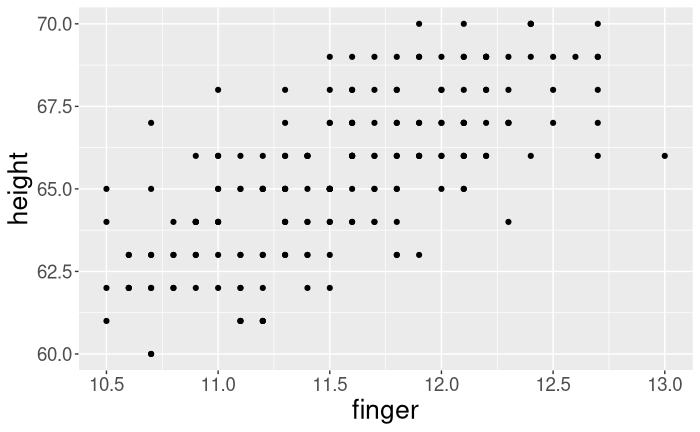
\includegraphics[scale = 0.4]{example1_SRS.png}
  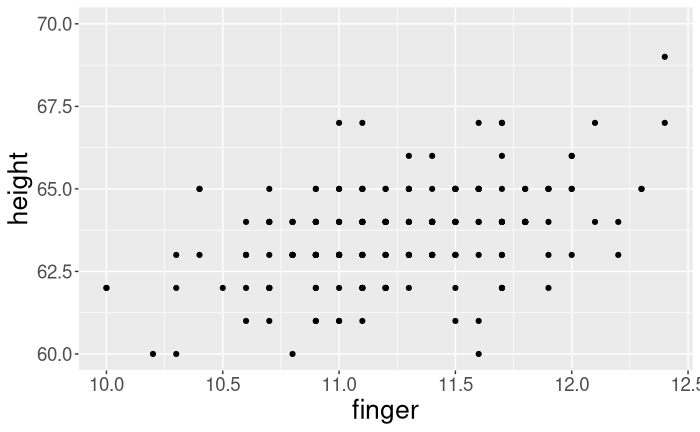
\includegraphics[scale = 0.4]{example1_UNEQ.png}
  \caption{Two samples from the api dataset. Left: Every person has the same
    probability of being included in the sample. Right: The probability of being
  included in the sample varies with the height.}
\end{figure}


This means that fitting a linear regression model to the unequal probabilities
sample will result in the slope tending to be smaller than what it should be, since there are few observations in the top right of the plot.

This will be illustrated now by fitting both a naive linear model and a model that takes into account the sampling probabilities.


% Code and plot of regression lines
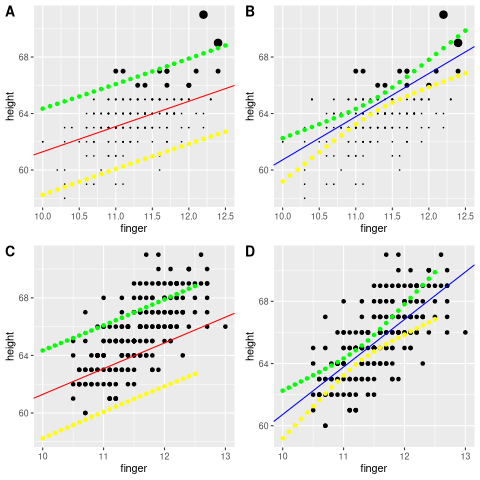
\includegraphics[scale = 0.5]{example1.png}

\textbf{Er noe feil med prediksjonsintervallet, det er altfor lite.}
\textbf{Skal gjøre plottene bedre.}


In this plot the points representing the observations have a radius proportional to the inverse of the sampling probability, so as you can see the observations in the top have a much smaller chance of being chosen that the ones in the bottom part. The red line is the regression line fitted by normal linear regression while the blue line is fitted by a model which takes the design into account. 

The blue line has a larger slope than the red line, indicating it gives the points in the top a bigger "weight" than the points in the bottom part to account for their lower sampling probabilities.

The top plots show the regression lines on top of the unequal probability sample.
The bottom plots show the regression lines on top of a sample where every
observation has an equal probability of being included.

We can see that the blue line fits better with the data than the red line in the
bottom plots.

\end{example}

\subsection{Data we are going to use}

The examples illustrating the theory will mostly use one dataset to illustrate the concepts
discussed. This is a dataset on the performance of students in schools in
California. This dataset has data on all 6194 schools with more than 100
students in California, with data collected
including: API scores in 1999 and 2000, which level of school it is
(elementary, middle, high), name of school, location of school, percentage of
students tested at the school, API targets, economic factors for students at the
school, class sizes, information of education of parents and qualification of teachers.

API scores is a metric testing the academic performance of the students at the school.

We will use this data as the population we will sample from, and we will take
different kinds of samples to illustrate the concepts introduces in this thesis.

The thesis will start by giving an introduction to survey statistics, where giving the necessary background theory needed to be able to talk about linear regression in this context.

\section{Introduction survey statistics}

There are two big differenses between ``normal'' statistics and Survey statistics.

The first difference is that in Survey statistics you approach the ''randomness'' from a different angle.
Usually in statistics you let individual values be stochastic variables
with some distribution and one observation is a sample from that stochastic
variable.

In Survey statistics on the other hand you say that the individual values are
fixed, i.e. my height is not random, every time you measure it you will get the
exact same result, if you discount measurement errors. Instead what is random is
who we sample. This leads us to a couple definitions:

\begin{definition} \label{def:sampUnit}
  A \textbf{sampling unit} is one "element" we want to sample. In the case of
  our API example this will be one school.
\end{definition}

\begin{definition} \label{def:sampPop}
The \textbf{sampling population}, or universe, \(U = \{1, 2, 3, ..., N\}\), is a
finite set containing all the sampling units you are interested in. In our case
it will be all the schools in California having 100 or more students.
\end{definition}

To represent the elements in \(U\) by natural numbers we just let the elements
have a arbitrary ordering and denote them by their indices. We do this for
simplicity of notation as the order of the elements do not matter in the inference.

\begin{definition} \label{def:sampFrame}
The \textbf{sampling frame} is the list of all sampling units you are going to sample from. Ideally the sampling frame and the sampling population would be the same, but that is not always to case. In some cases for example, you may not have a list of all the people who are eligible to vote, you may perhaps only have a list of the people who voted in the last election. This can cause a bias in the results.
\end{definition}

In the API case, the sampling population and the sampling frame are equal, since
we have a table of all the data and we will just choose rows from that table for
our samples. But there are cases where this is not the case. An example of this
could be if we were doing a political survey to try to predict who will win the
next election.
In that case our sampling population, who we are interested in information
about, would be everyone who are going to vote in the next election. It is
is impossible to get a list of them though, so we instead have to use choose
some other part of the population we have information about. We might have a
list of all who voted last election, which might be a good approximation of
those who are going to vote this election, but then we would miss out on all the
new eligible voters and people who might have decided to vote this election but
didn't do it the last one.

Choosing the correct sampling frame to match your target sampling population is
difficult and getting it wrong can make your results wrong.


\begin{definition} \label{def:sample}
A \textbf{sample}, \(S \subseteq U\), is a subset of the sampling frame. This is the data we will analyse to try to get information about the sampling population.
\end{definition}

We will denote the sampling units chosen in the sample by their indices in the
sampling population.

\begin{definition} \label{def:probSample}
A \textbf{probability sample} is a sample where the elements sampling units included are chosen randomly.
\end{definition}

\begin{definition} \label{def:sampProb}
The \textbf{sampling probability} of a sampling unit is the probability that a specific sampling unit is included in the sample.
\end{definition}

So we have a probability sample, where every sampling unit has some probability to be included in the sample, called the sampling probability.


The other big difference is that normally you assume that you sample from an
infinity population which has some distribution. In Survey statistics however we
have a finite distribution which means that it no longer makes sense thinking
about it having a distribution. This means that we no longer need the assumption
of which distribution the sampling units come from. This gives us more freedom,
and less potential problems if our assumptions are wrong.


The goal of Survey statistics is generally to estimate some statistic of the whole
population from a sample. These statistics include the total of some value,
f.eks. the total number of students in school, the mean of some value, f.eks.
the mean number of students per teacher in school, or to estimate regression
coefficients to either do inference or predict future values.

I will first start by talking about different kinds of samples along with some
inference on some statistics calculated from these samples and then finish with
talk about regression.

\section{Model based simple linear regression} \label{sec:modLinReg}

We will first give a short summary of normal simple linear regression, in a
model based context. We have a response variable, \(y\), and a predictor, \(x\). The
relationship between \(y\) and \(x\) is assumed to be:

\begin{equation*}
Y = \beta_0 + \beta_1 x + \epsilon,
\end{equation*}
where \(\epsilon\) is a stochastic error term.

I.e. we assume there exists \(\beta_0\) and \(\beta_1\) that describes this
relationship perfectly.
We do not know these values however, so we instead have to estimate them given
independent observed data points. We call these data points \((x_1, y_1), (x_2, y_2)
... (x_n, y_n)\). To do
this we want to find \(\hat{\beta}_0\) and \(\hat{\beta}_1\) that minimize the
Residual Sum of Squared (RSS). The RSS is defined by:

\begin{align*}
  RSS &= \frac{1}{n} \sum_{i = 1}^N \left( y_i - \hat{y}_i \right)^2 
  = \frac{1}{n} \sum_{i = 1}^N \left( y_i - \hat{\beta}_0 - \hat{\beta}_1 x_i \right)^2
\end{align*}

The \(\hat{\beta}_0\) and \(\hat{\beta}_1\) that minimizes the RSS are:
%$$
%\hat{\beta}_1 = \frac{\sum_{i = 1}^N\left( x_i - \bar{x} \right) \left( y_i -
    %\bar{y} \right)} {\sum_{i = 1}^N \left( x_i - \bar{x} \right)}
%$$
%and
%$$
%\hat{\beta}_0 = \bar{y} - \hat{\beta}_1 \bar{x}
%$$

\begin{equation*}
 \hat{\beta_1} = \frac{\sum_{i = 1}^n\left( x_i - \bar{x} \right) y_i}{\sum_{i = 1}^n\left( x_i - \bar{x} \right)} 
\end{equation*}

\begin{equation*}
 \hat{\beta_0} = \bar{y} - \hat{\beta_1}\bar{x} 
\end{equation*}

Under some conditions it's shown that these estimates are the best estimates
you can get for \(\beta_0\) and \(\beta_1\). These conditions are:

\begin{enumerate}
\item \(E \left( \epsilon_i \right) = 0\ \forall \ i = 1, 2, ..., n\)
\item \(Var \left( \epsilon_i \right) = \sigma^2\ \forall \ i = 1, 2, ..., n\)
\item All the \(\epsilon\) are independent of any predictor or observation number.
\item All \(\epsilon_1\), \(\epsilon_2\), ..., \(\epsilon_n\) are independent of each other.
\end{enumerate}

If all these assumption are followed get that the estimates are unbiased and:
\begin{equation*}
  Var \left( \hat{\beta}_0 \right) = \sigma^2 \frac{\sum_{i = 1}^N x_i^2}{n
    \sum_{i = 1}^N \left( x_i - \bar{x} \right)^2}
\end{equation*}
  

\begin{equation*}
  Var \left( \hat{\beta}_1 \right) = \frac{\sigma^2}{
    \sum_{i = 1}^N \left( x_i - \bar{x} \right)^2}
\end{equation*}

\section{Regression in the context of finite populations}

In the case of finite populations things change a bit. We still want to find the
coefficients that minimize the RSS, but since the population is finite our goal
is to find the line that minimizes the RSS for the whole population, i.e. find
\(B_0\) and \(B_1\) such that \(\sum_{i = 1}^N (y_i - B_0 - B_1 x_i)\) is as small as
possible.

If we know the whole population we can just compute them using the same formulas
as in Section \ref{sec:modLinReg}, which if we rewrite them we get:

\begin{equation*}
  B_0 = \frac{1}{N} \left( t_y - \frac{t_{xy} t_x - \frac{1}{N} t_y t_x^2}
    {t_{x^2} - \frac{1}{N} t_x^2}
   \right)
\end{equation*}

\begin{equation*}
  B_1 = \frac{t_{xy} - \frac{1}{N} t_y t_x}
    {t_{x^2} - \frac{1}{N} t_x^2}
\end{equation*}

If we let \(t_x = \sum_{i = 1}^N x_i\), \(t_y = \sum_{i = 1}^N y_i, t_{x^2} =
\sum_{i = 1}^N x_i^2\) and \(t_{xy} =
\sum_{i = 1}^N x_i y_i\).


The case where we know the whole population however is not that interesting, we are instead interested in the case where we have to sample from the
population to estimate such statistics.

If we then let \(\hat{t}_x, \hat{t}_y, \hat{t}_{x^2}, \hat{t}_{xy}, \hat{N}\) be estimators
for \(t_x, t_y, t_{x^2},
t_{xy}, N\) respectively we get the estimators for \(B_0\) and \(B_1\):

\begin{equation*}
  \hat{B}_1 = \frac{\hat{t}_{xy} - \frac{1}{\widehat{N}} \hat{t}_y \hat{t}_x}
    {\hat{t}_{x^2} - \frac{1}{\widehat{N}} \hat{t}_x^2}
\end{equation*}

\begin{equation*}
  \hat{B}_0 = \frac{1}{\widehat{N}} \left( \hat{t}_y - \frac{\hat{t}_{xy} \hat{t}_x - \frac{1}{\widehat{N}} \hat{t}_y \hat{t}_x^2}
    {\hat{t}_{x^2} - \frac{1}{\widehat{N}} \hat{t}_x^2}
  \right)
  = \frac{\hat{t}_y}{\hat{N}} - \hat{B}_1\frac{\hat{t}_x}{\hat{N}}
\end{equation*}

It gets very complicated calculation variance for these estimators, so we ofter
try to estimate them instead. There are several ways to do so, but a common on
and the one we will use in here is linearization. Linearization takes a
non-linear expression of stochastic variables we can do inference about and uses
the first two terms of the Taylor expansion to make it linear.
Say for example we have \(h(a, b, c, d, e) = \frac{ea - bc}{ed - b^2}\), such that
\(h(\hat{t_{xy}}, \hat{t_x}, \hat{t}_y, \hat{t}_{x^2}, \hat{N}) = \hat{B_1}\).

We therefore have that
\begin{align*}
  Var(\hat{B_1})
  &= Var \left( h(\hat{t_{xy}}, \hat{t_x},
  \hat{t}_y, \hat{t}_{x^2}, \hat{N})) \right) \\
  &\approx Var \left(h(t_{xy}, t_x, t_y,
t_{x^2}, N) + \frac{\partial h} {\partial(a, b, c, d, e)} (t_{xy}, t_x, t_y,
t_{x^2}, N) * (\hat{t_{xy}}, \hat{t_x}, \hat{t}_y, \hat{t}_{x^2}, \hat{N}) - (t_{xy}, t_x, t_y,
t_{x^2}, N) \right) \\
    &= Var\left( \frac{\partial h}{\partial a}(t_{xy}) * (\hat{t_{xy}} - t_{xy}) + \frac{\partial h}{\partial b}(t_{x}) * (\hat{t_{x}} - t_{x}) +  \frac{\partial h}{\partial c}(t_{y}) * (\hat{t_{y}} - t_{y}) + \frac{\partial h}{\partial d}(t_{x^2}) * (\hat{t_{x^2}} - t_{x^2}) + \frac{\partial h}{\partial e}(N) * (\hat{N} - N) \right)
\end{align*}

\subsection{Simple random sample}

One of the simpler probability samples is a Simple Random Sample (SRS). A
sample of size \(M \leq N\) is an SRS if every subset \(S \subseteq U\) has the same
probability of being chosen.

Lets say for example that \(U = \{1, 2, 3, 4\}\) and that we want a sample, \(S\) of
size \(3\). Then there are \(\binom{4}{3} = 4\)  possible samples of size \(3\):

\begin{equation*} S_1 = \{1, 2, 3\} \end{equation*}
\begin{equation*} S_2 = \{1, 2, 4\} \end{equation*}
\begin{equation*} S_3 = \{1, 3, 4\} \end{equation*}
\begin{equation*} S_4 = \{2, 3, 4\} \end{equation*}.

For this to be a SRS each of these subsets need to have the same probability of
being chosen, i.e. \(P(S_1) = P(S_2) = P(S_3) = P(S_4) = 0.25\). A consequence of
having a SRS is that all the sampling probabilities are all equal, \(P(1 \in S) =
P(2 \in S) = P(3 \in S) = P(4 \in S) = 0.75\). But having equal sampling
probabilities is not sufficient for the sample to be an SRS.

Look for example at this case:
Assume we want a sample of size \(2\) from a population of size \(4\), and that
\(P(\{1, 3\}) = 0.5\) and \(P(\{2, 4\}) = 0.5\) while the probabilities of all the
other possible samples are \(0\). Then \(P(1 \in S) = P(2 \in S) = P(3 \in S) = P(4 \in S) = 0.5\)
but this is not a SRS since all possible subsets of size \(2\) do not have equal
probability of being chosen.


\subsection{Estimation}

One of the more common statistics we want to estimate is the total of some value
for the whole population. We might for example want to estimate the total number
of students enrolled in school, in our API example.

We would then denote the value of interest in one school, i.e. the number of
enrolled students by \(y_i\) and let
\begin{equation*}
  t_y = \sum_{i = 1}^{N} y_i
\end{equation*}
be the value we want to estimate.

The natural estimate of this total, if we sample \(n\) elements, would be
\begin{equation*}
\hat{t}_y = \frac{N}{n}\sum_{i \in S} y_i
\end{equation*}
where we take the average of the values in our sample and then scale it up to
the whole population.

It can be shown using indicator variables and sampling probabilities that
\(\hat{t}_y\) is an unbiased estimator for \(t_y\).


A statistic related to the total is the mean of some value. We denote the true
mean in the population
\begin{equation*}
\bar{y}_U = \frac{1}{N} \sum_{i = 1}^{N} y_i
\end{equation*}
and the sample mean
\begin{equation*}
\bar{y}_S = \frac{1}{n} \sum_{i \in S} y_i ,
\end{equation*}
which we use as our estimator.

Then we can rewrite the estimate for \(t\) as:
\begin{equation*}
\hat{t}_y = \frac{N}{n} \sum_{i \in S} y_i = N\bar{y}_S
\end{equation*}

Using the fact that \(\hat{t}_y\) is unbiased it is trivial to show that
\(\bar{y}_S\) is an unbiased estimator for \(\bar{y}_U\).

It can be shown that the variance of the estimator is of the form:
\begin{equation*}
Var \left( \bar{y}_S \right) = \frac{S^2}{n} \left( 1 - \frac{n}{N}
\right)
\end{equation*}

where

\begin{equation*}
S^2 = \frac{1}{N - 1} \sum_{i = 1}^N (y_i - \bar{y}_U)^2
\end{equation*}

is the variance of the whole population.

We do not, however, know \(S^2\) as that would require us to know to \(y\) values
for the whole population \(U\). Instead we estimate \(S^2\) by:

\begin{align*}
  s^2
  &= \frac{1}{n - 1} \sum_{i \in S} \left( y_i - \bar{y}_S \right)^2
\end{align*}

which gives us the estimate of \(Var(\bar{y}_U)\):
\begin{align*}
  \widehat{Var(\bar{y}_U)}
  &= \frac{1}{n} \left( 1 - \frac{n}{N} \right) s^2
\end{align*}

Since \(s^2\) is unbiased we have that \(\frac{s^2}{n} \left( 1 - \frac{n}{N}
\right)\) is an unbiased estimator of the variance of \(\bar{y}_S\).

From this it follows that the variance of \(\hat{t}_S\) has the unbiased estimator
\(\frac{N^2}{n} s^2 \left( 1 - \frac{n}{N} \right)\).

The factor \(\left( 1 - \frac{n}{N} \right)\) in the variances is what differs in
these variance estimates compared to the ``normal'' ones. It is called the
\textbf{finite population coefficient (fpc)} and comes from the fact that we are
sampling without replacement from a finite population.

When we sample a larger and larger portion on the population we will get more
and more information and therefore the variance will decrease towards zero. This
means that if we sample half the population the variance estimate will be half
of the variance estimate in model based statistics.


\subsection{Stratification}

\subsection{Clustering}

\subsection{Complex surveys}

\subsection{Variance estimation (?)}




\end{document}
